\section[Rational Herglotz derivatives and an exponentially small oscillation]{Rational Herglotz derivatives\\and an exponentially small oscillation}
\label{sec:herglotz}

Let
\[
 F(x)=\sum_{n\ge1}\frac{\psi(nx)-\log(nx)}n,\qquad
 D_r(x)=\frac{(-1)^{r+1}x^{r+1}}{r!}F^{(r)}(x)
 \quad(r\ge1, x>0).
\]
The all-orders assertion that rational jets reduce to depth-one cyclotomic
polylogarithms is already stated by Radchenko--Zagier~\cite{RZ}, immediately after
Proposition~4 of their preprint, p.~9. It must not be presented as a new
closure theorem. The explicit Bernoulli coefficient formula below gives a
constructive version; the large-order estimate and its effective remainder
bound are derived independently here. The limit considered below is derivative order tending to infinity at a fixed positive argument.

\subsection{An explicit finite rational-jet formula}

Write $B_j(X)$ for the Bernoulli polynomials with $B_1(X)=X-1/2$.
For positive integers $p,q$ (coprimality is unnecessary for this formula), put
\[
 c_{a,b}=\frac aq+\frac bp,\qquad
 d_{r,j}(a,b)=\binom rj B_{r-j}(1-b/p)
              -\mathbf1_{j=0}B_r(a/q),
\]
where $1\le a\le q$, $0\le b<p$, and $0\le j<r$.

\begin{theorem}[Finite Bernoulli--Hurwitz evaluator]\label{thm:rational-jets}
For $r\ge1$,
\begin{align*}
F^{(r)}(p/q)
={}&\frac{(-1)^{r+1}(r-1)!q^{r-1}}{p^{r+1}}
\left\{
\sum_{a=1}^{q}\sum_{b=0}^{p-1}
\left[-\psi(c_{a,b})+
 \sum_{j=0}^{r-1}d_{r,j}(a,b)\zeta(r+1-j,c_{a,b})\right]
\right.\\[-2pt]
&\hspace{50mm}\left.{}+pq\left(\frac1r-\gamma-\log q\right)
\right\}.
\end{align*}
In particular every Hurwitz zeta value in the formula has integer order
between $2$ and $r+1$; no spectral derivatives occur.
\end{theorem}

\begin{proof}
Use the classical integral representation (Radchenko--Zagier, eq.~(6))
\[
 F^{(r)}(x)=(-1)^{r+1}
 \int_0^\infty t^r\operatorname{Li}_{1-r}(e^{-xt})
 \left(\frac1{1-e^{-t}}-\frac1t\right)dt.
\]
After $t=qu$ introduce, initially for $\Re s>0$,
\[
 I(s)=\int_0^\infty u^{r+s}\operatorname{Li}_{1-r}(e^{-pu})
 \left(\frac1{1-e^{-qu}}-\frac1{qu}\right)du.
\]
The combined integral is holomorphic on $\Re s>-1$ since its integrand is
$O(u^{\Re s})$ at zero. In $\Re s>0$ the two terms can be integrated
separately, giving
\[
 I(s)=\Gamma(r+1+s)
 \sum_{n\ge1,m\ge0}\frac{n^{r-1}}{(pn+qm)^{r+1+s}}
 -\frac{\Gamma(r+s)}{qp^{r+s}}\zeta(1+s).
\]
Set $n=qk+a$, $m=p\ell+b$, and $h=k+\ell$. Faulhaber's identity gives
\[
 \sum_{k=0}^h(qk+a)^{r-1}
 =\frac{q^{r-1}}r
 \left[B_r(h+1+a/q)-B_r(a/q)\right].
\]
Writing $v=h+c_{a,b}$ expands the bracket as
$\sum_{j=0}^r d_{r,j}(a,b)v^j$, with $d_{r,r}=1$.
Consequently
\[
 \sum_{n\ge1,m\ge0}\frac{n^{r-1}}{(pn+qm)^{r+1+s}}
 =\frac{q^{r-1}}{r(pq)^{r+1+s}}
 \sum_{a,b}\sum_{j=0}^r d_{r,j}(a,b)
 \zeta(r+1+s-j,c_{a,b}).
\]
The $j=r$ terms have Laurent expansion
$\zeta(1+s,c)=s^{-1}-\psi(c)+O(s)$.
Their combined residue cancels that of the second term of $I(s)$.
The finite part of the two gamma factors contributes
$pq[1/r-\gamma-\log q]$ after factoring out
$(r-1)!/(p^{r+1}q^2)$. Finally
$F^{(r)}(p/q)=(-1)^{r+1}q^{r+1}I(0)$.
All rearrangements took place in an absolutely convergent half-plane;
holomorphy of the combined integral justifies taking the finite part.
\end{proof}

\paragraph{Cyclotomic interpretation.}
For coprime $p,q$, the rational function
\[
 R_{r,p,q}(z)=\frac{\operatorname{Li}_{1-r}(z^p)}{1-z^q}
\]
has poles only at $p$th and $q$th roots of unity. Its coefficient sequence
has a unique finite decomposition
\[
 [z^N]R_{r,p,q}(z)=
 \sum_{\omega^p=1\ \text{or}\ \omega^q=1}
 \sum_{j=0}^{r}a_{\omega,j}N^j\omega^N\quad(N\ge1).
\]
The coefficients lie in $\mathbb Q(\mu_{pq})$,
$a_{1,r}=1/(rp^rq)$, and $a_{\omega,r}=0$ for $\omega\ne1$.
Partial fractions therefore give the equivalent formula
\[
 F^{(r)}(p/q)=(-1)^{r+1}(r-1)!(q/p)^r
 \left(\frac1r+\log p\right)
 +(-1)^{r+1}r!q^{r+1}
 \sum_{\omega}\sum_{j=0}^{r-1}
 a_{\omega,j}\operatorname{Li}_{r+1-j}(\omega).
\]
This proves the already known closure statement and gives all its
coefficients. The special $a_{1,r}\zeta(1+s)$ term is the only pole:
its finite-part contribution is exactly the displayed elementary term.

For example,
\begin{align*}
 F''(1)&=-\frac12-\zeta(2),&
 F'''(1)&=\frac23+3\zeta(2)+\zeta(3),\\
 F''(1/2)&=-2-8\zeta(2)-\frac72\zeta(3),&
 F'''(1/2)&=\frac{16}3+48\zeta(2)+32\zeta(3).
\end{align*}
At $p=q=1$ the complete formula reduces to
\[
 F^{(r)}(1)=(-1)^{r+1}(r-1)!
 \left[\frac1r+
 \sum_{j=1}^{r-1}\binom rj B_{r-j}(1)\zeta(r+1-j)\right].
\]
For high $r$ this exact expression can suffer substantial floating-point
cancellation; exact coefficients do not make low-precision evaluation
reliable.

\subsection{The complete algebraic large-order expansion}

Define
\[
 E_r(x)=D_r(x)-\zeta(2)-\frac xr(\log x-H_{r-1}).
\]
The following result concerns $r\to\infty$ with $x$ fixed, not the
large-$x$ Bernoulli expansion of $F$.

\begin{theorem}[Large derivative order with effective remainder]\label{thm:herglotz-bound}
For $x>0$, integers $r\ge2$, real $1<A<r$, and
$\pi/4<\theta<\pi/2$,
\begin{align*}
 |E_r(x)|\le{}&
 \frac{2x\zeta(A)\zeta(A+1)}
 {\pi(2\theta-\pi/2)\cos\theta}
 \left(\frac{x}{2\pi\cos^2\theta}\right)^A
 \frac{\Gamma(r-A)\Gamma(A)\Gamma(A+1)}{\Gamma(r+1)}.
\end{align*}
Consequently, uniformly for $x$ in each compact subinterval of $(0,\infty)$,
\[
 E_r(x)=O\left(r^{-1/2}\exp[-2\sqrt{\pi r/x}]\right).
\]
In particular, the exact harmonic-number expression
$\zeta(2)+(x/r)(\log x-H_{r-1})$ contains every algebraic order in $1/r$.
\end{theorem}

\begin{proof}
Binet's digamma integral and Mellin inversion give, for $1<c<2$,
\[
 F(x)+\frac{\zeta(2)}{2x}
 =-\frac1{2\pi i}\int_{c-i\infty}^{c+i\infty}
 \frac{\pi\Gamma(s)\zeta(s)\zeta(s+1)}
 {(2\pi x)^s\sin(\pi s/2)}\,ds.
\]
One derivation is to Mellin-transform
$\psi(y)-\log y+1/(2y)$ in $1<\Re s<2$ using
$\int_0^\infty v^{s-1}/(1+v^2)\,dv=\pi/[2\sin(\pi s/2)]$;
the sum over $n$ supplies $\zeta(s+1)$. Absolute convergence of Binet's
integral and exponential decay on vertical lines justify inversion and
fixed-order differentiation. After $r$ differentiations,
\[
 D_r(x)=\frac{\zeta(2)}2+
 \frac1{2\pi i}\int_{(c)}
 \frac{\pi\Gamma(r+s)\zeta(s)\zeta(s+1)x^{1-s}}
 {\Gamma(r+1)(2\pi)^s\sin(\pi s/2)}\,ds.
\]
Move the contour to $\Re s=-A$. The only crossed poles are $s=1$ and
$s=0$. At the negative even integers the zero of $\zeta(s)$ cancels
the sine denominator; gamma poles lie to the left since $A<r$.
The residue at $1$ is $\zeta(2)/2$. Using
$\zeta'(0)=-\tfrac12\log(2\pi)$ and
$\psi(r)=H_{r-1}-\gamma$, the residue at $0$ is
$x(\log x-H_{r-1})/r$.
Thus the integral on the new line equals $E_r(x)$.

Apply the zeta functional equation twice to its kernel:
\[
 \frac{\pi\zeta(s)\zeta(s+1)}
 {(2\pi)^s\sin(\pi s/2)}
 =2(2\pi)^s\cos(\pi s/2)
 \Gamma(1-s)\Gamma(-s)\zeta(1-s)\zeta(-s).
\]
On $s=-A+it$, use
$|\zeta(1-s)\zeta(-s)|\le\zeta(A+1)\zeta(A)$ and
$|\Gamma(r-A+it)|\le\Gamma(r-A)$.
Rotating the Euler gamma integral through angle
$\theta\operatorname{sgn}(t)$ gives the elementary inequality
\[
 |\Gamma(a+it)|\le
 \Gamma(a)(\cos\theta)^{-a}e^{-\theta|t|}
 \qquad(a>0, 0<\theta<\pi/2).
\]
Use it for the other two gamma factors, with parameters $A$ and $A+1$,
and use $|\cos(\pi s/2)|\le e^{\pi|t|/2}$.
The remaining integral is
$\int_{\mathbb R}e^{-(2\theta-\pi/2)|t|}dt
=2/(2\theta-\pi/2)$, yielding the stated effective bound.
The same estimates justify the horizontal-contour limits.

For the stretched-exponential estimate take an integer
$m=\sqrt{\pi r/x}+O(1)$ and $\theta=\pi/4+1/(2m)$.
For $r$ sufficiently large, $1<m<r$ and the bound applies.
Uniformly on compact positive $x$-intervals,
\[
 \frac{\Gamma(r-m)}{\Gamma(r+1)}
 =r^{-m-1}\exp\left[\frac{m(m+1)}{2r}+O(r^{-1/2})\right],
 \qquad
 \Gamma(m)\Gamma(m+1)=2\pi m^{2m}e^{-2m}(1+O(m^{-1})).
\]
Also
$(2\pi\cos^2\theta)^{-m}=\pi^{-m}e^{1+O(m^{-1})}$,
and the prefactor is $O(xm)$. The power and exponential factors reduce
to $O(r^{-1/2}e^{-2\sqrt{\pi r/x}})$, as required.
\end{proof}

\paragraph{An elementary factorial form.}
At $\theta=\pi/3$ and integer $2\le m<r$ the estimate becomes
\[
 |E_r(x)|\le \frac{24x}{\pi^2}\zeta(m)\zeta(m+1)
 \left(\frac{2x}{\pi}\right)^m
 \frac{(r-m-1)!(m-1)!m!}{r!}.
\]
It is useful as a directly computable error certificate even without
asymptotic optimization.

\paragraph{Positivity and a convergent Taylor certificate.}
The derivative integral has a positive kernel with
$1/2<1/(1-e^{-t})-1/t<1$, so
\[
 \frac{\zeta(2)}2<D_r(x)<\zeta(2).
\]
Therefore the Taylor expansion of $F(x+h)$ about $x>0$ has, for
$\rho=|h|/x<1$, the explicit remainder bound
\[
 \left|F(x+h)-\sum_{j=0}^{N}\frac{F^{(j)}(x)}{j!}h^j\right|
 \le\frac{\zeta(2)}x\frac{\rho^{N+1}}{1-\rho}.
\]
Its radius is exactly $x$, since $D_r(x)\to\zeta(2)$.

\subsection{Exact arithmetic sectors and the leading oscillation}

The divisor-weighted eta/Binet representation in Radchenko--Zagier~\cite[Section~7.3]{RZ} is classical context for this calculation. The following identity is a differentiated and reciprocity-transformed form useful for large derivative order. The quantitative sum estimates are needed in addition to a one-sector expansion.


Write $\sigma_{-1}(n)=\sum_{d\mid n}d^{-1}$. Let $U$ denote Tricomi's
confluent hypergeometric function with its principal branch. Its integral
representation is DLMF~13.4.4~\cite{DLMF}. The large-first-parameter asymptotics used
below are classical (DLMF~13.8.11--16; Temme~\cite{Temme}); a direct saddle calculation
is included to fix the branch and the first correction in this application.
The arithmetic sum over all sectors and its aggregate error bound must be
justified in addition to that classical one-sector asymptotic.

\begin{theorem}[Exact divisor-weighted expansion]\label{thm:herglotz-sectors}
For every integer $r\ge2$ and $x>0$,
\begin{align*}
 E_r(x)
 &=2x\Gamma(r)\sum_{n\ge1}\sigma_{-1}(n)
       \Repart U\left(r,0,\frac{2\pi i n}{x}\right)\\
 &=2x\sum_{n\ge1}\sigma_{-1}(n)
   \int_0^\infty\frac{u^{r-1}}{(1+u)^{r+1}}
        \cos\left(\frac{2\pi n u}{x}\right)du.
\end{align*}
The series of the integrals is absolutely convergent. The assertion does
not require absolute convergence after moving the infinite sum inside
the oscillatory $u$-integral.

More precisely, for $1<A<r$ and $\pi/4<\theta<\pi/2$, the contribution
of an arbitrary subset $\mathcal N\subset\mathbb N$ is bounded by the
previous effective estimate with $\zeta(A)\zeta(A+1)$ replaced by
$\sum_{n\in\mathcal N}\sigma_{-1}(n)n^{-A}$.
\end{theorem}

\begin{proof}
Set $w=-s$ in the post-functional-equation contour representation:
\[
 E_r(x)=\frac{2x}{2\pi i\Gamma(r+1)}
 \int_{(A)}\Gamma(r-w)\Gamma(w)\Gamma(w+1)
 \zeta(w)\zeta(w+1)\cos(\pi w/2)
 \left(\frac{x}{2\pi}\right)^w dw.
\]
The Dirichlet series
$\zeta(w)\zeta(w+1)=\sum_{n\ge1}\sigma_{-1}(n)n^{-w}$
converges absolutely on this line. The effective gamma bound proves
absolute convergence of the resulting series of contour integrals.

For $\Re z>0$ put
\[
 M_r(z)=\int_0^\infty e^{-zu}
        \frac{u^{r-1}}{(1+u)^{r+1}}du=\Gamma(r)U(r,0,z).
\]
For $0<\Re w<r$, taking its Mellin transform in $z$ gives
\[
 \int_0^\infty z^{w-1}M_r(z)\,dz
 =\frac{\Gamma(w)\Gamma(r-w)\Gamma(w+1)}{\Gamma(r+1)}.
\]
Mellin inversion is valid in that strip. Both the defining integral
and the Barnes integral extend continuously to $z=\pm i\tau$, $\tau>0$:
the first by dominated convergence, since its rational weight is
integrable, and the second by its exponential vertical decay. Averaging
the two boundary values replaces $z^{-w}$ by
$\tau^{-w}\cos(\pi w/2)$. Substitution proves the formula and the
termwise bounds.
\end{proof}

\paragraph{A finite-sum tail bound.}
For an integer cutoff $N\ge1$ and $A>1$,
\[
 \sum_{n>N}\sigma_{-1}(n)n^{-A}
 \le N^{1-A}\left[\frac{1+\log N}{A-1}
                       +\frac1{(A-1)^2}\right],
\]
because $\sigma_{-1}(n)\le H_n\le1+\log n$ and
$(1+\log t)t^{-A}$ is decreasing for $t\ge1$.
Thus the exact series comes with a computable truncation bound.

An alternative bound avoids the auxiliary contour parameters.
Rotate the defining \(u\)-integral for \(M_r(i\tau)\) to the negative
imaginary ray. There are no poles in that quadrant; the small and
large arcs vanish. Then
\[
 |M_r(i\tau)|
 \leq\int_0^\infty e^{-\tau y}
       \frac{y^{r-1}}{|1-iy|^{r+1}}\dd y
 \leq\Gamma(r)\tau^{-r}.
\]
It follows that the arithmetic tail after \(N\) terms is at most
\begin{equation}\label{eq:herglotz-simple-tail}
 2x\Gamma(r)\left(\frac{x}{2\pi}\right)^r N^{1-r}
 \left(\frac{1+\log N}{r-1}+\frac1{(r-1)^2}\right),
 \qquad r\geq2.
\end{equation}
This is often the simplest finite-sum certificate; the earlier
gamma-factor bound is more useful for the sharp large-\(r\) exponent.

\begin{theorem}[Two-term oscillatory asymptotic]\label{thm:herglotz-oscillation}
For fixed $x>0$ define
\begin{align*}
 \mathcal A_r(x)&=
 2^{5/4}\pi^{3/4}x^{3/4}r^{-3/4}
       e^{-2\sqrt{\pi r/x}},\\
 \Phi_r(x)&=2\sqrt{\pi r/x}-\frac\pi x-\frac\pi8,\\
 \kappa(x)&=\frac3{16}\sqrt{\frac{x}{2\pi}}
             +\frac1{12}\left(\frac{2\pi}{x}\right)^{3/2}.
\end{align*}
Then, uniformly for $x$ in compact subintervals of $(0,\infty)$,
\[
 E_r(x)=\mathcal A_r(x)
 \left[\cos\Phi_r(x)+\frac{\kappa(x)}{\sqrt r}
          \cos\left(\Phi_r(x)+\frac\pi4\right)
          +O(r^{-1})\right].
\]
This is an additive oscillatory expansion; a relative-error claim after
division by $\cos\Phi_r(x)$ would be invalid near its zeros.
\end{theorem}

\begin{proof}
We first prove, uniformly for $z=i\tau$ with $\tau$ in any compact
positive interval,
\begin{equation}\label{hergnew:eq:Uasymp}
 M_r(z)=\sqrt\pi\,z^{1/4}r^{-3/4}
 e^{z/2-2\sqrt{rz}}
 \left[1+\frac1{\sqrt r}
       \left(\frac3{16\sqrt z}-\frac{z^{3/2}}{12}\right)
       +O(r^{-1})\right].
\end{equation}
All powers use their principal values.

Rotate the $u$-contour in the integral defining $M_r(i\tau)$ to
argument $-\pi/4$. There are no poles in that quadrant. On the large
arc the rational factor is $O(R^{-2})$, while
$|e^{-i\tau u}|\le1$; a small arc of radius $\epsilon$ contributes
$O(\epsilon^r)$.
Hence the rotation is justified directly. Put
\[
 u=\sqrt{r/z}\,v,\qquad
 \lambda=\sqrt{rz},\qquad \epsilon=\sqrt{z/r}.
\]
This gives the exact representation
\[
 M_r(z)=\sqrt{z/r}\int_0^\infty v^{-2}
  \exp\left[-\lambda v-(r+1)\log(1+\epsilon/v)\right]dv.
\]
On any fixed compact positive $v$-interval,
\begin{align*}
 -\lambda v-(r+1)\log(1+\epsilon/v)
 ={}&-\lambda(v+v^{-1})+\frac{z}{2v^2}\\
 &+r^{-1/2}\left(-\frac{\sqrt z}{v}
                    -\frac{z^{3/2}}{3v^3}\right)+O(r^{-1}),
\end{align*}
with the same estimates after any fixed number of $v$-derivatives.

For completeness, localization at $v=1$ is uniform. Write
$a=\sqrt{\tau/(2r)}$, so $\epsilon=a(1+i)$ and
$\Re\lambda=ra$. On a compact $v$-interval the real part of the
exponent is $-ra(v+v^{-1})+O(1)$, and $v+v^{-1}$ has its unique
minimum $2$ at $1$. For the small tail $0<v<\delta<1/2$, use
$|1+\epsilon/v|\ge1+a/v$ and substitute $y=a/v$:
\[
 \int_0^\delta v^{-2}|1+\epsilon/v|^{-r-1}dv
 \le\frac1{ar}(1+a/\delta)^{-r}
 =O\left(r^{-1/2}e^{-ra/\delta+O(1)}\right).
\]
This is exponentially smaller than $e^{-2ra}$.
For $v>M>2$, the factor $e^{-\lambda v}$ gives the analogous
bound $O(e^{-Mra})$. The remaining compact interval outside any
fixed neighborhood of $1$ also has a strict exponential gap.

Apply complex Laplace expansion at $v=1$ to
$\phi(v)=v+v^{-1}$ and
$g(v)=v^{-2}e^{z/(2v^2)}$.
It is legitimate since $\arg\lambda=\pi/4$ lies strictly inside
the right half-plane. The Gaussian integral along the real $v$-axis
gives $e^{-2\lambda}\sqrt{\pi/\lambda}$.
The coefficient of $1/\lambda$, divided by $g(1)$, is
\[
 \frac{g''(1)}{4g(1)}+\frac{3g'(1)}{4g(1)}+\frac3{16}
 =z+\frac{z^2}4+\frac3{16}.
\]
Adding the explicit $r^{-1/2}$ correction in the exponent at $v=1$
gives
\[
 -\sqrt z-\frac{z^{3/2}}3
 +\frac1{\sqrt z}\left(z+\frac{z^2}4+\frac3{16}\right)
 =\frac3{16\sqrt z}-\frac{z^{3/2}}{12}.
\]
This proves \eqref{hergnew:eq:Uasymp}; further terms follow by the same
finite Taylor and Gaussian-moment calculation, with standard local
remainder estimates. As an independent classical check, in DLMF~13.8.11
with $b=0$ one has $p_0(z)=1$ and $q_0(z)=-z/12$; the standard large-argument
expansions of $K_1$ and $K_0$ give exactly the same first correction.

At $z=2\pi i/x$, taking $2x$ times the real part of
\eqref{hergnew:eq:Uasymp} gives the stated main term and correction.
Indeed $z^{1/4}$ has argument $\pi/8$, and the correction equals
$\kappa(x)e^{-\pi i/4}$.

It remains to control all the other arithmetic sectors uniformly.
For $A\ge2$,
\[
 \zeta(A)\zeta(A+1)-1
 =\sum_{n\ge2}\sigma_{-1}(n)n^{-A}
 \le 4\bigl(\zeta(2)\zeta(3)-1\bigr)2^{-A}.
\]
Use the effective sector bound with
$A=\sqrt{2\pi r/x}+O(1)$ an integer and
$\theta=\pi/4+1/(2A)$. Exactly the previous optimization yields
\[
 \sum_{n\ge2}2x\sigma_{-1}(n)\Repart M_r(2\pi i n/x)
 =O\left(r^{-1/2}e^{-2\sqrt{2\pi r/x}}\right).
\]
This is absorbed into $\mathcal A_r(x)O(r^{-1})$, uniformly on compact
positive $x$-intervals.
\end{proof}

\begin{corollary}[Sharp exponential rate and infinitely many signs]\label{cor:herglotz-signs}
For each fixed $x>0$ the real sequence $E_r(x)$ takes positive and
negative values infinitely often. More precisely,
\[
 \limsup_{r\to\infty}\frac{E_r(x)}{\mathcal A_r(x)}=1,
 \qquad
 \liminf_{r\to\infty}\frac{E_r(x)}{\mathcal A_r(x)}=-1,
\]
and
\[
 \limsup_{r\to\infty}\frac{\log|E_r(x)|}{\sqrt r}
 =-2\sqrt{\pi/x}.
\]
Here $\log0=-\infty$ if an exact zero occurs.
\end{corollary}
\begin{proof}
The phase $\Phi_r(x)$ increases to infinity, with successive differences
tending to zero. Consequently it has subsequences approaching any fixed
phase modulo $2\pi$. Apply the additive expansion and choose phases
$0$ and $\pi$. The same subsequences establish the lower bound for the
limsup of the logarithmic rate; the asymptotic envelope gives the upper
bound.
\end{proof}

\paragraph{Further research specific to this section.}
Compute and certify several further half-integer corrections in
\eqref{hergnew:eq:Uasymp}; build an interval implementation of the exact
sector sum; locate the sign-transition indices beyond the leading
$\sqrt r$ phase law; and obtain a uniform transition theory when $x$
also varies with $r$. The fixed-$x$ theorem above does not justify such
a double-scaling limit automatically.


\begin{figure}[t]
\centering
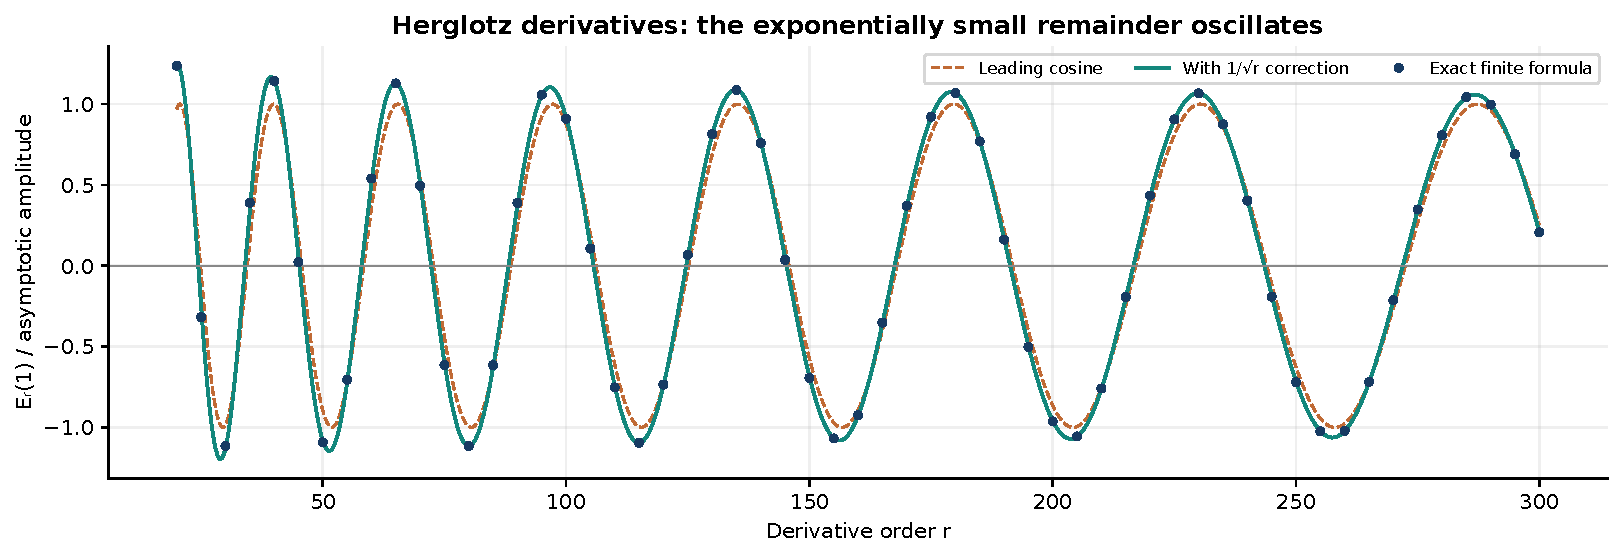
\includegraphics[width=\textwidth]{figures/herglotz_oscillation.pdf}
\caption{The Herglotz remainder divided by its asymptotic amplitude at $x=1$. The leading cosine and its first correction track the exact finite-formula values. The asymptotic is additive, so no division by a small cosine is used.}
\label{fig:herglotz}
\end{figure}
